\chapter{Vyhodnocení}

V této kapitole popisujeme v sekci~\ref{methods} způsob vyhodnocení našeho systému,
v sekci~\ref{results} výsledky tohoto vyhodnocení a v sekci~\ref{improvements}
vylepšení, která jsme na základě výsledků navrhli, spolu s nápady k jejich implementaci.

\section{Způsob vyhodnocení}\label{methods}

Běžné způsoby vyhodnocení dialogových systémů zaměřených na plnění úkolů popisují
\citet[podsekce 24.5.2]{jurafsky_slp_2020}. Primárním měřítkem je poměr úspěšně
splněných úkolů. U jiných druhů úkolů, kde je potřeba vyplnit více slotů, je možné
sledovat ještě podrobněji poměr správně vyplněných slotů, ale náš systém
vyplňuje pouze jméno, tedy řešit poměr splněných úkolů je dostatečné.

Vytvořili jsme dotazník, v jehož úvodu jsme popsali náš systém a způsob instalace
aplikace, a následně se uživatelů dotazovali především na počet pokusů o hovor a
množství úspěšných zahájení hovoru. Dále nás zajímaly konkrétnější důvody neúspěšných
pokusů o hovor, návrhy na vylepšení a celkový zájem o takovou aplikaci. Dotazník je
možné najít v příloze TODO .

\section{Výsledky}\label{results}

Podařilo se nám získat \(15\) testovacích uživatelů, kteří dohromady uskutečnili 91
pokusů o hovor, z toho \(51\) bylo úspěšných, jak znázorňuje
graf na obrázku~\ref{img-ratio-succ}. Celková úspěšnost
systému tedy byla \(56\,\rm \%\).

Velmi zajímavý je zájem o podobnou aplikaci, který znázorňuje graf na obrázku~\ref{img-ratio-interest}.
Pouze \(20\,\rm \%\) uživatelů uvedlo, že by o takovou aplikaci nemělo vůbec zájem.
Zbylí by o takovou aplikaci měli zájem, pokud by fungovala lépe, přidala nové funkce,
případně oboje.

% \begin{figure}[h]
%     \centering
%     \subfloat[Graf úspěšnosti splnění úkolu.]%
%     {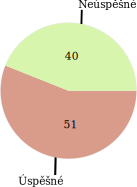
\includegraphics[width=0.28\textwidth]{../img/chart-succ.pdf}}
%     \hfill%
%     \subfloat[Graf zájmu o podobnou aplikaci.]%
%     {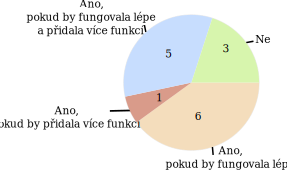
\includegraphics[width=0.6\textwidth]{../img/chart-interest.pdf}}
% \end{figure}

\newsavebox{\tempbox}
\begin{figure}[H]
    \sbox{\tempbox}{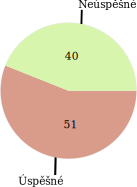
\includegraphics[width=0.28\textwidth]{../img/chart-succ.pdf}}
    \subfloat[Úspěšnost plnění.]{\usebox{\tempbox}\label{img-ratio-succ}}%
    \qquad
    \subfloat[Zájem o podobnou aplikaci.]{\vbox to \ht\tempbox{%
            \vfil
            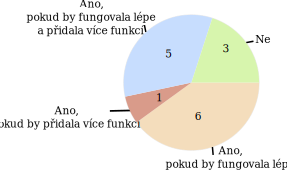
\includegraphics[width=0.6\textwidth]{../img/chart-interest.pdf}
            \vfil}\label{img-ratio-interest}}%
    \caption{Grafy výsledků.}
\end{figure}

Co se týká konkrétnějších důvodů selhání, největším problémem bylo nalezení více
kontaktů a nezdařený výběr z nich. Dalšími častými problémy bylo nerozpoznání
jména ve WA, nalezení neodpovídajících kontaktů a špatně rozpoznaná řeč.

Nutnou opravou je z pohledu uživatelů lepší rozpoznávání jmen i přiřazování
kontaktů k nim, za důležité také zmínili potvrzení vytáčení ještě jedním
\uv{ano/ne}. Několikrát byla zmíněna také plynulost aplikace a rychlost
odpovědi.
Nejvíce žádaným vylepšením byla schopnost rozpoznávat libovolný název kontaktu
místo čistě jmen, mnoho uživatelů využívá názvy kontaktů \uv{Mamka} a podobné.
Několikrát zmíněným vítaným vylepšením by také byla schopnost posílat textové
zprávy.

\section{Vylepšení a jejich možná implementace}\label{improvements}

V této sekci se budeme zabývat nutnými a možnými vylepšeními, která
vyplynula z vyhodnocení s uživateli. V podsekci~\ref{better-match}
uvedeme návrhy na zlepšení porovnávání uživatelova vstupu s jeho
seznamem kontaktů. V podsekci~\ref{better-app} pak navrhneme
úpravy v aplikaci, které by vedly k lepšímu uživatelskému
zážitku, pokud by cílem bylo čistě vytáčení kontaktů.

\subsection{Zkvalitnění přiřazování}\label{better-match}

Největším problémem bylo přiřazování názvů kontaktů spolu s neschopností přiřadit
názvy, které nejsou českými jmény. Z hlediska implementačního se o tuto část
stará WA, naše porovnávací komponenta pracuje až s entitami rozpoznanými jím.
Jako možná řešení vidíme rozšířit základnu entit, se kterými WA pracuje. Ke
každému jménu bychom mohli získat domácké formy (jako \uv{Honza} ke jménu \uv{Jan})
a přidat je do WA, kromě nich ještě běžné názvy rodinných příslušníků,
které uživatelé často využívají jako názvy kontaktů (\uv{Mamka}, \uv{Babička}).
Pro zpřesnění bychom mohli přidat i relevantní vyskloňované tvary jmen (ke jménu \uv{Jan}
také \uv{Janu}, \uv{Janovi}, \uv{Jana}).

Další možností by bylo snažit se v této omezené doméně hledat jmenné entity na
základě vzorců, když uživatel říká \uv{zavolej}, obvykle následuje název
kontaktu.

Poslední možností je přepracovat porovnávací komponentu, aby nebyla závislá
na entitách rozpoznaných pomocí WA. Touto cestou se pravděpodobně vydáme,
protože nám dává největší volnost implementace a především velkou
použitelnost mimo konkrétní doménu.

\subsection{Přepracování mobilní aplikace}\label{better-app}

Velká většina uživatelů uvedla, že by o aplikaci měli zájem, pokud by fungovala
lépe, i kdyby nepřidala další funkce. V takovém případě bychom se obešli
bez celé detekce úmyslů a mohli celý dialog velmi zjednodušit.

Navrhovaný běh představujeme v ukázce níže. Uživatel by stiskem
tlačítka zapnul rozpoznávání řeči a řekl jen název kontaktu,
kterému chce zavolat. Celý tento vstup by byl přímo v zařízení
porovnán se všemi názvy kontaktů v seznamu, pravděpodobně za
využití knihovny \texttt{JavaWuzzy}.\footnote{https://github.com/xdrop/fuzzywuzzy} Pokud by byl
nalezen jeden ostře lépe odpovídající kontakt, aplikace
by oznámila úmysl mu volat a uživatel by potvrdil \uv{ano/ne}.
Pokud by odpovídalo více kontaktů, ale méně než 4, uživatel
by z nich dostal na výběr. Pokud by jich bylo více, dostal by
žádost o zpřesnění požadavku. Celou dobu by bylo možné slovem
\uv{znovu} či obdobným začít od začátku.
\begin{code}
    Uživatel: /Stiskne tlačítko/
    Systém:   /Začne naslouchat/
    Uživatel: Název Kontaktu
    Systém:   /Porovnává celý vstup s kontakty přímo v zařízení/
    Systém:   Chcete zavolat Název Kontaktu?
    Uživatel: Ano
    Systém:   /Zahájí hovor/
\end{code}

Tím, že by celé řízení dialogu i porovnání mohlo probíhat v aplikaci,
dosáhli bychom větší plynulosti aplikace, neboť bychom nemuseli čekat
na vyřízení síťových požadavků. Zjednodušením by se celý dialog také
výrazně zrychlil, což je žádoucí, protože zahájení hovoru by mělo
být rychlé.

Ideální variantou by pak bylo kdyby i rozpoznání a generování řeči
dokázalo běžet lokálně v aplikaci bez nutnosti kontaktování serveru.
Celá aplikace by pak mohla běžet offline. Zde by mohl pomoci projekt
\texttt{DeepSpeech}.\footnote{https://github.com/mozilla/DeepSpeech}
Nutností by bylo získat dostatek trénovacích dat v češtině. Vytvořením
otevřených datasetů v mnoha jazycích se zabývá projekt Common Voice \citep{commonvoice_2020},
kam může kdokoliv dobrovolně přispět.